\documentclass{article}

\usepackage[brazil]{babel}
\usepackage[utf8]{inputenc}
\usepackage{amsmath}

\usepackage{listings}
\usepackage{mcode}
\usepackage[section]{placeins}

\usepackage{graphicx}

\usepackage{color} %red, green, blue, yellow, cyan, magenta, black, white
\definecolor{mygreen}{RGB}{28,172,0} % color values Red, Green, Blue
\definecolor{mylilas}{RGB}{170,55,241}

\begin{document}

\begin{flushleft}
FUNDAÇÃO GETÚLIO VARGAS \\

Escola de Pós-Graduação em Economia

Teoria Macroeconômica III

Professor: Ricardo de Oliveira Cavalcanti

Monitora: Kátia Aiko Nishiyama Alves

Alunos: Gustavo Bulhões e Samuel Barbosa
\end{flushleft}

\section*{Exercício 01}
Neste exercício temos um modelo de search no mercado de trabalho com as seguintes funções/parâmetros:

\begin{lstlisting}
f = @(w, alpha_1, alpha_2) alpha_1 + alpha_2 * w;
u = @(c, gamma) c .^ gamma;

beta = 0.98;
pi = 0.1;
b = 0;
wmin = 0;
wmax = 20;
gamma = 1/2;
\end{lstlisting}

\subsection*{Item (i)}

No item (i) vamos usar que $f(0) = 2f(\overline{w})$. 
Como $\int_{0}^{\overline{w}} f(w) dw = 1$, resolvemos para $\alpha_1, \alpha_2$ e obtemos:

\begin{lstlisting}
alpha_1 = 1/15;
alpha_2 = -1/600;
\end{lstlisting}

Neste modelo o agente escolhe entre aceitar uma oferta de trabalho a um salário $w$ ou 
continuar procurando por uma oferta no próximo período a um salário $w'$. 
Escrevemos o problema do agente na forma recursiva, e resolvemos para obter a função 
valor $V(w)$, a função política $G(w)$ e o preço de reserva $R$ do agente 
(o salário que o torna indiferente entre aceitar ou não uma oferta de trabalho).

Para aproximar numericamente a função valor, criamos um grid para a variável de estado $w$, 
entre 0 e 20, contendo $n = 1000$ pontos, e aplicamos aplicamos um algoritmo de iteração 
buscando o ponto fixo do operador 

$$T(V)(w) = \underset{I(w) \in \{0,1\}}{max} I(w) \{u(w) + \beta [(1-\pi) V(w) + \pi V(0)] \} + [1-I(w)] [u(b) + \beta E[V(w')]].$$

\newpage
\begin{lstlisting}
n = 1000;
w = linspace(wmin, wmax, n)';
V = ones(n, 1); % chute inicial para a funcao valor
G = ones(n, 1); % chute inicial para a funcao politica

% inicia variaveis do algoritmo de iteracao
err = 1;
tol = 10^-5;
itmax = 2000;
iter = 1;

% fdp discretizada e funcao valor esperado
fw = f(w, alpha_1, alpha_2) ./ sum(f(w, alpha_1, alpha_2));
E = @(fw, V, n) V' * fw; 
\end{lstlisting}

Definimos $N$ como o payoff de recusar uma oferta $w$ e seguir a política ótima a partir do próximo período, 
e $A$ como o payoff de aceitar $w$ e seguir a política ótima a partir do próximo período. 
Deste modo o algoritmo de iteração é dado por

\begin{lstlisting}
% algoritmo de iteracao
while err > tol && iter < itmax
    N = u(b, gamma) + beta * E(fw, V, n);
    N = repmat(N, n, 1);
    A = u(w, gamma) + beta * ((1-pi) * V + pi * N);
    [TV, G] = max([N A], [], 2);
    err = abs(max(TV - V));
    V = TV;
    iter = iter + 1;
end

G = G-1;
R = min(w(G == 1));
\end{lstlisting}

Utilizado o código descrito obtemos $R \approx 8.8288$ e as seguintes funções valor e política:

\begin{figure}[!h]
  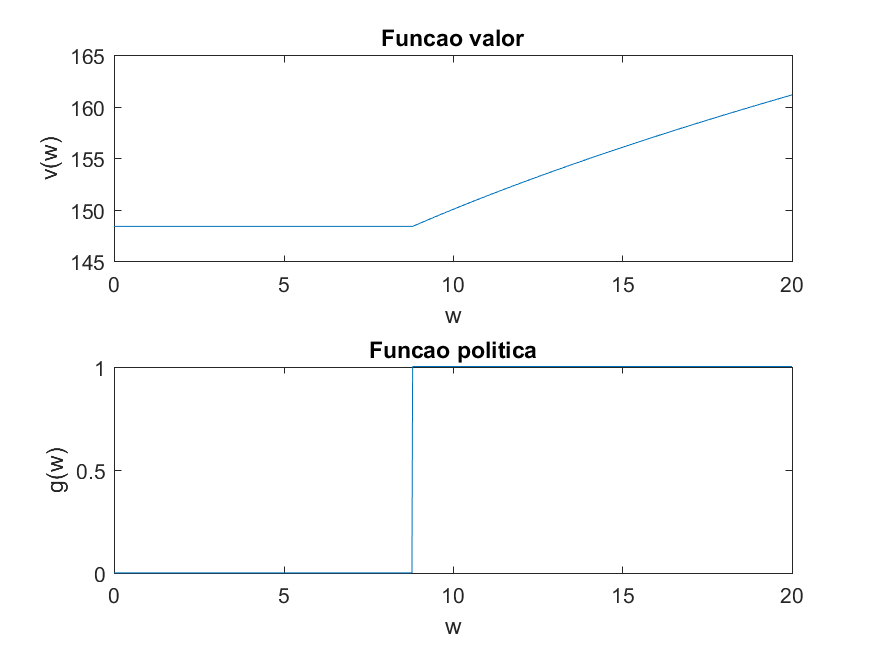
\includegraphics{ex1_1.png}
\end{figure}

\section*{Item (ii)}

No item (ii) refazemos o exercício usando $f(\overline{w}) = 2f(0)$ em oposição a $f(0) = 2f(\overline{w})$ tal como no item (i).
Agora obtemos 

\begin{lstlisting}
alpha_1 = 1/30;
alpha_2 = 1/600;
\end{lstlisting}

A distribuição de $w$ passa a ter maior densidade em valores mais altos,
implicando em maior probabilidade de ofertas de trabalho com salários maiores.
Aplicando o algoritmo para os novos valores de  $\alpha_1$ e $\alpha_2$, 
obtemos $R \approx 10.3904$, e as funções valor e política se alteram para

\begin{figure}[!h]
  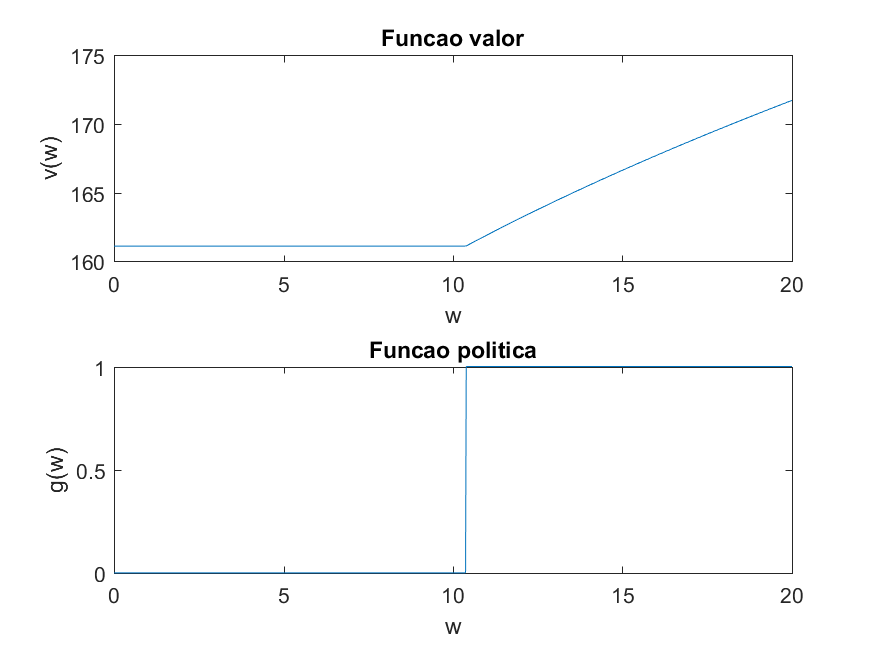
\includegraphics{ex1_2.png}
\end{figure}

\end{document}